\documentclass[mathserif,18pt,xcolor=table]{beamer}

\usepackage {bbm}
\usepackage {textpos}

\definecolor{utorange}{RGB}{203,96,21}
\definecolor{utblack}{RGB}{99,102,106}
\definecolor{utbrown}{RGB}{110,98,89}
\definecolor{utsecbrown}{RGB}{217,200,158}
\definecolor{utsecgreen}{RGB}{208,222,187}
\definecolor{utsecblue}{RGB}{127,169,174}

\mode<presentation>
{
  % \usetheme{Pittsburgh}   
  \usetheme{Boadilla}  
  %\usefonttheme[onlymath]{serif}
  \usefonttheme[stillsansseriftext]{serif}

  \setbeamercovered{invisible}
  \setbeamertemplate{navigation symbols}{}

  % Color Theme 
    \setbeamercolor{normal text}{bg=white,fg=utblack}
  \setbeamercolor{structure}{fg=utorange}

  \setbeamercolor{alerted text}{fg=red!85!black}

  \setbeamercolor{item projected}{use=item,fg=black,bg=item.fg!35}

  \setbeamercolor*{palette primary}{use=structure,fg=white, bg=utorange}
  \setbeamercolor*{palette secondary}{use=structure,bg=utsecbrown}
  \setbeamercolor*{palette tertiary}{use=structure,bg=utsecgreen}
  \setbeamercolor*{palette quaternary}{use=structure,fg=structure.fg,bg=utsecblue}

  % \setbeamercolor*{frametitle}{use=structure,fg=utorange, bg=utsecbrown}
  \setbeamercolor*{framesubtitle}{fg=utbrown}

  \setbeamercolor*{block title}{parent=structure,fg=black,bg=utsecgreen}
  \setbeamercolor*{block body}{fg=black,bg=utblack!10}
  \setbeamercolor*{block title alerted}{parent=alerted text,bg=black!15}
  \setbeamercolor*{block title example}{parent=example text,bg=black!15}

  \setbeamerfont{framesubtitle}{size=\small}
}

\usepackage[orientation=landscape,size=custom,width=16,height=9.75,scale=0.5,debug]{beamerposter}
% \usepackage[orientation=landscape,size=custom,width=16,height=9,scale=0.5,debug]{beamerposter}


\makeatletter
\setbeamertemplate{footline}
{
  \leavevmode%
    \hbox{%
      \begin{beamercolorbox}[wd=.333333\paperwidth,ht=2.25ex,dp=1ex,center]{author in head/foot}%
        \usebeamerfont{author in head/foot}\insertshortauthor%~~\beamer@ifempty{\insertshortinstitute}{}{(\insertshortinstitute)}
      \end{beamercolorbox}%
        \begin{beamercolorbox}[wd=.333333\paperwidth,ht=2.25ex,dp=1ex,center]{title in head/foot}%
        \usebeamerfont{title in head/foot}\insertshorttitle
        \end{beamercolorbox}%
        \begin{beamercolorbox}[wd=.333333\paperwidth,ht=2.25ex,dp=1ex,right]{date in head/foot}%
        \usebeamerfont{date in head/foot}\insertshortdate{}\hspace*{2em}
        \insertframenumber{} / \inserttotalframenumber\hspace*{2ex} 
      \end{beamercolorbox}}%
        \vskip0pt%
}
\makeatother

\usepackage[T1]{fontenc}
\usepackage[protrusion=true,expansion=true]{microtype}
\usepackage{amsmath}


\renewcommand*{\thefootnote}{\fnsymbol{footnote}}


\pgfdeclareimage[height=1.0cm]{utbig}{logos/UTWordmark}
\pgfdeclareimage[height=0.6cm]{ut}{logos/UTWordmark}
\pgfdeclareimage[height=1.5cm]{sclogo}{logos/SC12}
% \pgfdeclareimage[height=1.0cm]{scsmall}{logos/SC12}

\hypersetup{
    colorlinks=true,
    linkcolor=blue,
    filecolor=magenta,
    urlcolor=cyan,
    pdftitle={Overleaf Example},
    pdfpagemode=FullScreen,
    }
    
\usepackage[T1]{fontenc}
\usepackage{lmodern}


\usepackage{graphicx}
\graphicspath{ {../multimedia/} }

\institute[UT, Austin]{University of Texas at Austin, PGE}

\title[Num modelling of salt caverns]{Numerical modelling of salt caverns}
\subtitle{Literature assessment, brainstorming}
\author[RPoli]{Renato Poli}
\date{November 12, 2023}

\begin{document}

\maketitle

\setbeamerfont{frametitle}{size=\small}
\setbeamerfont{framesubtitle}{size=\tiny}

\begin{frame}{Poromec - a 3D poroelastic solver with explicit fractures}
\begin{itemize}
	\item Poroelastic solver (non linear to cope with fracture flow)
	\item Validated with Terzaghi and mandel solution
	\item Validating now fracture mechanics (working good so far...)
	\item Non-structured. gmsh generates the mesh
	\item Integrated to cmake and parallel computing in LNCC (sdumont)
\end{itemize}
\vspace{10pt}
I am using the solver to a final project in geomechanics course.

The idea is to exercise homogeneization of mechanical and poroelastic parameters in a fractured media.
\end{frame}

\begin{frame}{IT Setup}
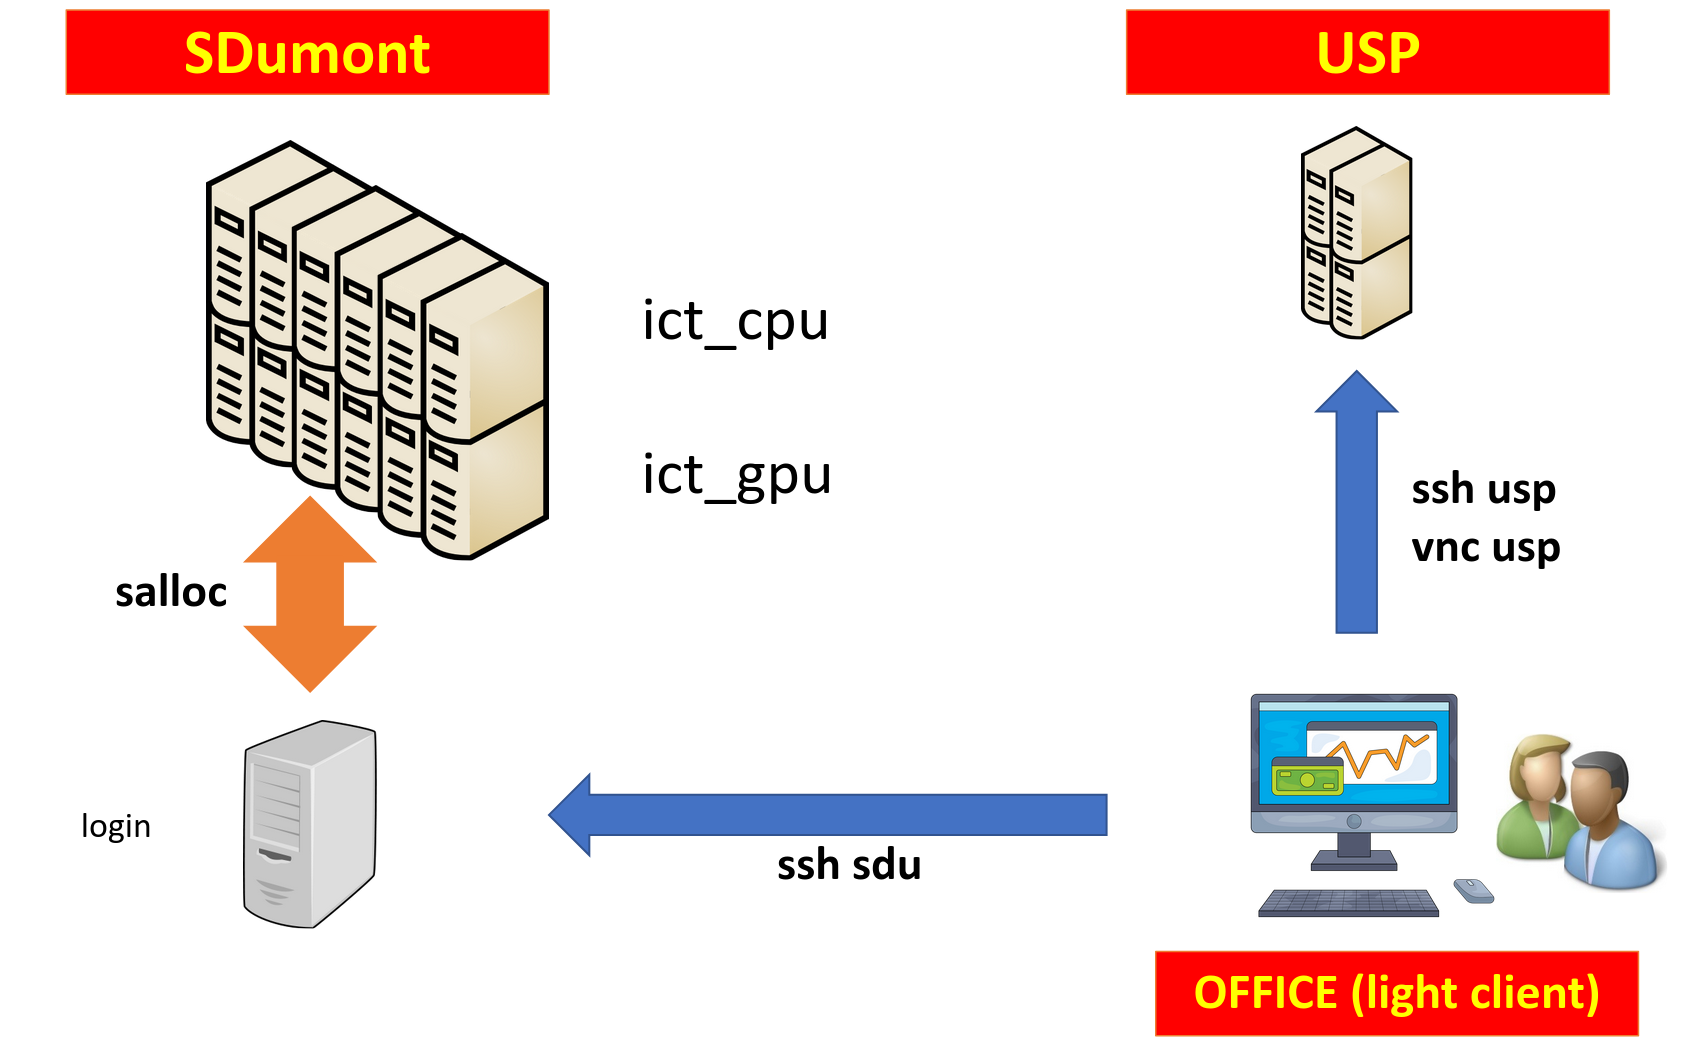
\includegraphics[width=13cm]{png/it_archit}
\end{frame}

\begin{frame}{Pure normal opening}
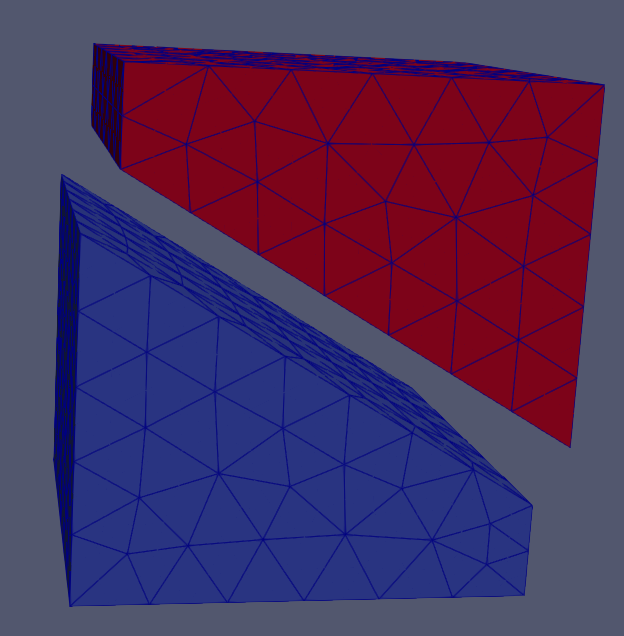
\includegraphics[width=9cm]{png/poromec-fracture-pure-normal}
\end{frame}

\begin{frame}{Pure shear opening}
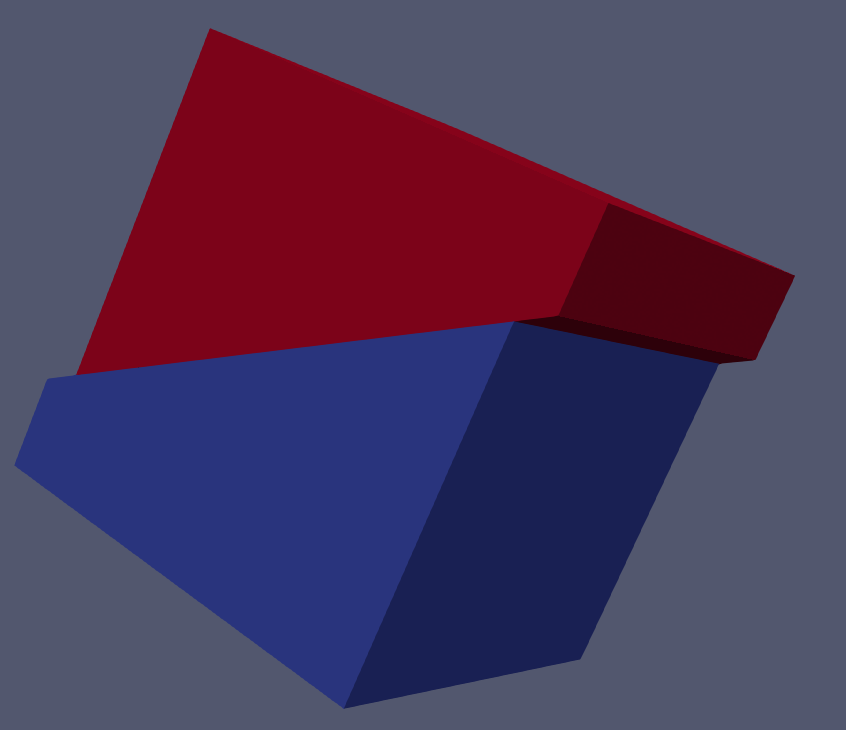
\includegraphics[width=9cm]{png/poromec-fracture-pure-shear}
\end{frame}

\begin{frame}{Mesh design - GMSH}
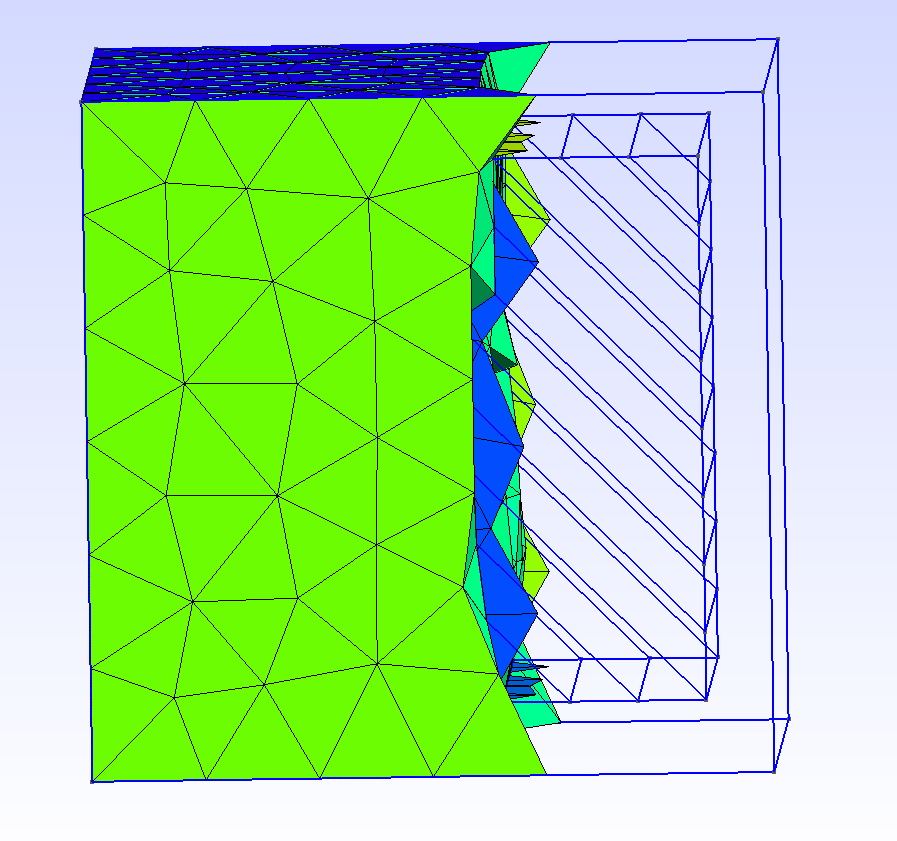
\includegraphics[width=9cm]{png/poromec-fracture-media}
\end{frame}

\begin{frame}{Dilated fractures}
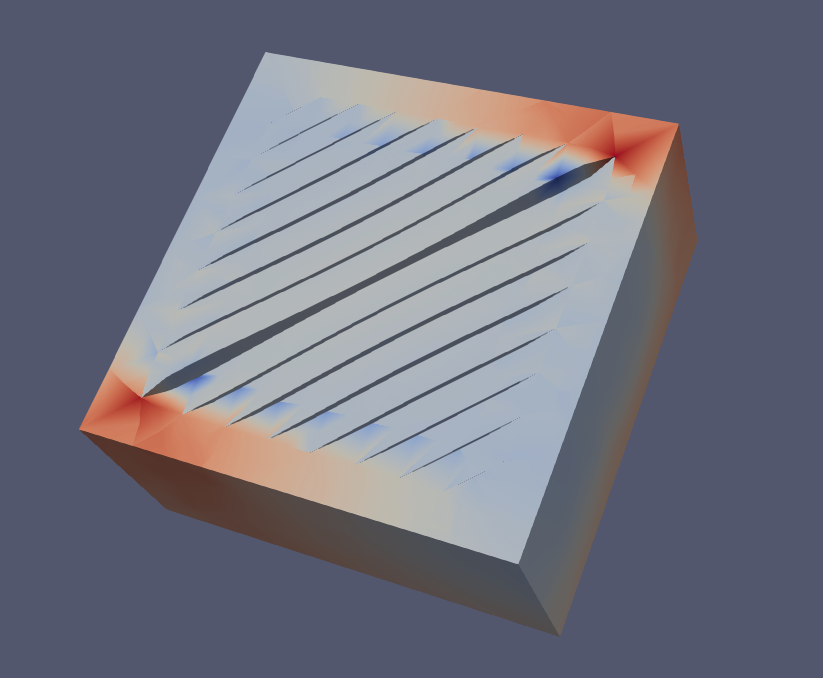
\includegraphics[width=9cm]{png/poromec-dilated-fractures}
\end{frame}

\begin{frame}[fragile]{Preliminary results}
\begin{verbatim}
E(input):1.70e+10
K(input):9.44e+09
K(output):5.59e+09
eps:5.17e-07
sxx:2.82e+03
syy:2.84e+03
szz:3.01e+03
sxy:-8.04e+00
syz:-5.70e-01
sxz:1.49e+00
sm:2.89e+03
tri_dx:1.03e-05
tri_dy:1.03e-05
tri_dz:5.29e-06
\end{verbatim}

\end{frame}

\begin{frame}{Ideation - overall goals and start narrowing}
\begin{itemize}
\item Cavern creation
	\begin{itemize}
	\item Chemical reaction
	\item Circulate fluid and model the size/shape of the cavern
	\end{itemize}
\item Volumetrics, cavern design
	\begin{itemize}
	\item Given a shape, what is the capacity
	\item Analytical approach or simple numerics will solve most cases (ref:\cite{maraggi23})
	\end{itemize}
\item Risks, legislation
	\begin{itemize}
	\item Geomechanics
	\item Well as a critical feature for leakage - modelling of cement, chemical reactivity, abandonment etc
	\end{itemize}
\item Numerics
	\begin{itemize}
	\item Complex models for salt creep
	\item Need to include plasticity
	\item Need data do calibrate (mechanical data for salt is not abundant - afaik)
	\item Large displacements need to be considered for long term creep
	\item Advanced computer architecture (GPUs, ...)
	\end{itemize}
\end{itemize}
\end{frame}


\begin{frame}{Workflow (still to fill...)}
\begin{itemize}
\item Understand the problem
	\begin{itemize}
		\item Overall picture
		\item Where it is applied
		\item Main challenges
		\item Accidents?
		\item Risks, regulations
    \end{itemize}
\item Prototype
	\begin{itemize}
		\item Proof of concepts - currently using PoroMec (own simulator)
		\item Standalone software
	\end{itemize}
\item Case study
	\begin{itemize}
		\item 
	\end{itemize}
\item Optimize
\end{itemize}
\end{frame}

\begin{frame}[shrink=20,fragile]{Talk to Hassan Abadi}
\begin{itemize}
\item A sponsor: \href{https://www.respec.com/market/energy/caverns-hydrogen-underground-storage/}{RESPEC website}
\item Impact of the cycles in stability
\item Low energy density of the caverns ($H_2$)
%\item MIT - Mechanical Integrity Test (using $N_2$)
%\item The brine in long contact with the cavern walls may impact stability?
\item Overview of projects worldwide? It seems that Canada has a well-set market on storage in caverns
%\item Muri Dussault (???) - Kamy knows him
\item Adcore - utility company in Canada?
\item The key of the research is risk and regulation (form companies and governments)
\item Percolation of H2 in water saturated rock.
\item Flow in caverns is in open space and mainly gravitational
\item Well is a critical point. Cement-rock interface, how to ensure seal? Wellbore is a critical point of leakage
%\item Tetsiana (Stanford) - talked about cement
\end{itemize}
\end{frame}

\begin{frame}{Lorena (UT @ Austin)}
\framesubtitle{\cite{maraggi23} Modeling hydrogen storage capacities, injection and withdrawal cycles in salt caverns: Introducing the GeoH2 salt storage and cycling app}
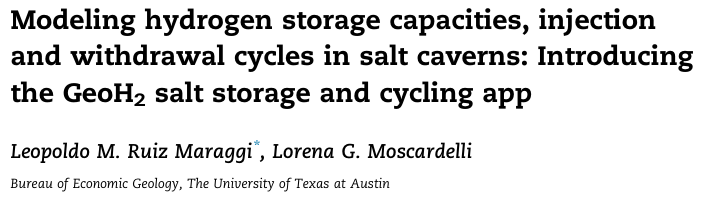
\includegraphics[width=10cm]{png/maraggi23}
\begin{itemize}
\item Presents the online tool GeoH\textsubscript{2} to calculate overall aspects of a salt cavern (volumetrics, pressure, flow rate etc).
\item Considers simple geometries (spherical, cylindrical)
\item Mainly analytical work
\item Discusses the physics involved
\item Does not assess risks and geomechanics
\item Conclusions could be more clear "there are \textit{many} (...) technical challenges that still need ..." sounds too generic (which challenges?)
\end{itemize}
\end{frame}

%
%
\begin{frame}{RCGI - Brazil}
\framesubtitle{\cite{goulart20} Technology readiness assessment of ultra-deep salt caverns for carbon capture and storage in Brazil}
\begin{itemize}
\item Funded by FAPESP RCGI (Research center for gas innovation - \href{https://sites.usp.br/rcgi/br/rgci_br/}{link}). Founder sponsors: Shell and Fapesp.
\item One of the authors is Alvaro Maia, a ex-Senior Consultant in Petrobras (well drilling, geomechanics).
\item They study caverns of up to 150x450m, created by dissolution, with geomechanical simulations.
\item Well is the critical element of an underground storage system, special attention to the cement.
\item May store 4 billion $Sm^3$
\item Used simulator COVES, developped by Alvaro Maia in the 1980s (See \cite{maia1984})
\end{itemize}
See also: \cite{abreu23}
\end{frame}
%
%
%
%
\begin{frame}[shrink=20, fragile]
\frametitle{PUCRIO - Investigation of well abandonment relying on salt creep}
\framesubtitle{\cite{firme23} - Geomechanics of salt towards natural barriers for the abandonment of pre-salt wells in Brazil}

\begin{columns}
\begin{column}{0.5\textwidth}
	\begin{itemize}
		\item Geomechanical study -- risk assessment.
		\item Proof of concept: can we abandon a well without cementing, just relying on natural closure after salt creep?
		\item 2D modelling of a well closure considering salt creep
		\item It seems to me that they used linear elastic, small strains FEM - which might not be good enough in this case
		\item Deviatoric stress up to 15MPa -- seems high to me, after creep
		\item Conclusion: creep takes too much time! (I think the study must be refined)
		\item EDMT - Enhanced Double Mechanism Creep Model (Pedro develloped during Phd - there's a thesis for that)
	\end{itemize}
\end{column}
\begin{column}{0.5\textwidth}  %%<--- here
    \begin{center}
     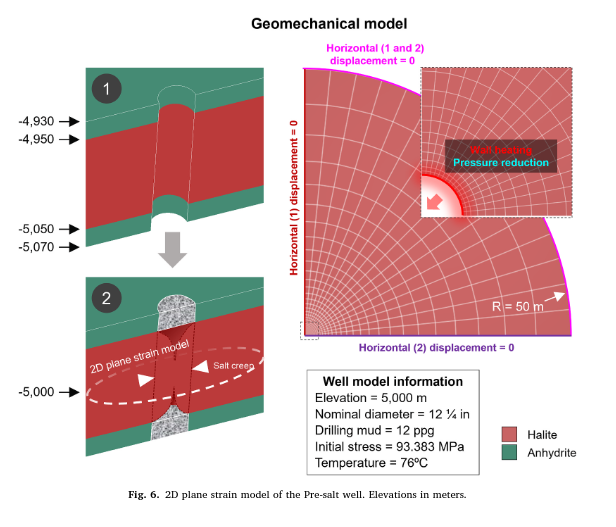
\includegraphics[width=\textwidth]{png/firme23}
     \end{center}
\end{column}
\end{columns}

\end{frame}
%
%

\begin{frame}{\cite{caglayan2020}Technical potential of salt caverns for hydrogen storage in Europe}
\end{frame}


\begin{frame}{\cite{li2021investigation} Investigation of thermal-mechanical effects on salt cavern during cycling loading}
Thermo-dependent salt creep. Thermo mechanical simulation. Pressure cycles, collapse and tensile fractures.
\end{frame}

\begin{frame}[shrink=30,fragile]{\cite{coarita23} Hydromechanical modelling of salt caverns subjected to cyclic hydrogen injection and withdrawal}
2D models, to consder cyclic loading, with fundamental creep and plasticity. Storage depths varying from 350 to 1350m. They claim the deeper is more mechanically unstable. They find the caverns are feasible.

Regarding formation of hydrogen plume (I could not completely understand the physics yet):
\begin{quote}
In addition to the hydromechanical modeqlling, an analysis of the
hydrogen extent within the rock mass is carried out. Since water and
hydrogen are immiscible, we assume hereafter that the threshold
capillary pressure of rock salt is much higher than hydrogen pressure
within the cavern due to the nanometric size of pore throats and hence
no free gas phase will be flowing. Assuming hydrogen is a non-reactive
solute (no chemical reaction or sorption with salt), we use the following
mass transport equation to delineate the extent and mass of dissolved
hydrogen plume. Transport of dissolved H2 is only driven by advection
(Darcy’s law) and by diffusion, since mechanical dispersion is negligible
due to the low permeability of the porous medium.
\end{quote}
\end{frame}

\begin{frame}{\cite{zhao22} Feasibility analysis of salt cavern gas storage in extremely deep formation: A case study in China}
\end{frame}
%\section{Goals of the caverns}
%\subsection{Energy storage}
%\begin{itemize}
%\item Regulate variations between renewable energy production and peak power demands (\cite{coarita23})
%\end{itemize}
%
%\subsection{Disposal}
%%\begin{itemize}
%%\end{itemize}
%
\begin{frame}{The physics behind}
I see concern with geomechanical behavior, targeted to creep, collapse and tensile fracturing. The cyclic behavior of the pressure is a significant difference compared to oil drainage and waterflooding.
\begin{itemize}
\item Geomechanics: creep, thermal, tensile fracture, shear fractures
\item Chemical: dissolution
\item Cyclic operations
\item Temperature dependent creep
\item Plume extension ($H_2$ dissolved in water - percolation of $H_2$ in water saturated rock (?))
\item Heat transfer, especially considering cyclic operations
\item Well integrity
\end{itemize}
\end{frame}

\begin{frame}[shrink=50,fragile]{References}
\bibliographystyle{apalike}
\bibliography{refs}
\end{frame}
\end{document}